\documentclass[a4paper,12pt]{report}
\usepackage{setspace}
\usepackage[a4paper, left=1.5in, right=1in, top=1in, bottom=1in]{geometry}
\usepackage{tikz}
\usetikzlibrary{shapes.geometric, arrows.meta, positioning}
\usepackage{graphicx}
\usepackage{fancyhdr}
\usepackage{float}
\usepackage{amsmath}
\usepackage{amssymb}
\usepackage{mathtools}
\usepackage{listings}
\usepackage{xcolor}
\usepackage{booktabs}
\usepackage{array}
\usepackage{longtable}
\usepackage{hyperref}

\hypersetup{
    colorlinks=true,
    linkcolor=black,
    urlcolor=blue,
    citecolor=black
}

% --- Color definitions ---
\definecolor{codebg}{RGB}{245,245,245}
\definecolor{codeframe}{RGB}{200,200,200}
\definecolor{keywordcolor}{RGB}{0,0,180}
\definecolor{commentcolor}{RGB}{80,80,80}
\definecolor{stringcolor}{RGB}{160,32,32}
\definecolor{accentblue}{RGB}{30,100,200}

% --- Code listing style ---
\lstset{
    language=Python,
    basicstyle=\ttfamily\small,
    keywordstyle=\bfseries,
    commentstyle=\itshape,
    stringstyle=\ttfamily,
    breaklines=true,
    frame=none,
    backgroundcolor={},
    numbers=left,
    numberstyle=\tiny\color{black},
    showstringspaces=false,
    tabsize=4,
    captionpos=b,
    xleftmargin=1.5em
}

% ==============================================================================
\begin{document}

% --- Title Page ---
\begin{titlepage}
\begin{center}

\Large
\textbf{VetAI -- AI-ENABLED DECISION SUPPORT SYSTEM FOR VETERINARIANS}

\vspace{1.5cm}

\large
A MAIN PROJECT REPORT\\[0.2cm]
submitted in partial fulfillment of the requirements for the award of the Degree of

\vspace{0.8cm}

\textbf{Master of Computer Applications}\\
UNDER\\
\textbf{APJ Abdul Kalam Technological University}

\vspace{1.5cm}

BY

\vspace{0.2cm}

\textbf{[YOUR NAME]}\\
[YOUR ROLL NUMBER]

\vspace{1.2cm}

\includegraphics[width=3cm]{mes.jpeg}

\vspace{1.2cm}

\textbf{DEPARTMENT OF COMPUTER APPLICATIONS}\\
[YOUR COLLEGE NAME]\\
[YOUR COLLEGE LOCATION]

\vfill

April 2026

\end{center}
\end{titlepage}

% --- Declaration ---
\thispagestyle{empty}
\begin{center}
\Large\textbf{Declaration}
\end{center}

\onehalfspacing
I undersigned hereby declare that the project report \textbf{VetAI -- AI-ENABLED DECISION SUPPORT SYSTEM FOR VETERINARIANS} submitted for partial fulfilment of the requirements for the award of degree of Master of Computer Applications of the APJ Abdul Kalam Technological University, Kerala, is a bonafide work done by me under supervision of \textbf{[Your Guide's Name]}, [Designation], Department of Computer Applications. This submission represents my ideas in my own words and where ideas or words of others have been included, I have adequately and accurately cited and referenced the original sources. I also declare that I have adhered to ethics of academic honesty and integrity and have not misrepresented or fabricated any data or idea or fact or source in my submission. I understand that any violation of the above will be a cause for disciplinary action by the institute and/or the University. This report has not been previously formed the basis for the award of any degree, diploma or similar title of any other University.

\vspace{3cm}

\noindent Date: [Date] \hfill
\begin{tabular}[t]{@{}r@{}}
[Your Name] \\[0.5cm]
[Your Roll Number]
\end{tabular}

\newpage

% --- Certificate ---
\thispagestyle{empty}
\begin{center}
\textbf{\Large [YOUR COLLEGE NAME]}\\[0.2cm]
\textbf{[YOUR COLLEGE LOCATION]}\\[0.2cm]
\small
(APPROVED BY AICTE AND AFFILIATED TO APJ ABDUL KALAM TECHNOLOGICAL UNIVERSITY )\\[1cm]
\includegraphics[width=80pt, height=80pt]{mes.jpeg}\\[1cm]
\textbf{\large DEPARTMENT OF COMPUTER APPLICATIONS}\\[1cm]
\textbf{\Large CERTIFICATE}\\[0.5cm]
\end{center}

\normalsize
\noindent
This is to certify that the project report entitled \textbf{VetAI -- AI-ENABLED DECISION SUPPORT SYSTEM FOR VETERINARIANS} is a bonafide record of the Main Project work during the academic year 2025--26 carried out by \textbf{[YOUR NAME] ([YOUR ROLL NUMBER])}, submitted to the APJ Abdul Kalam Technological University, in partial fulfilment of the requirements for the award of \textit{Degree of Master of Computer Applications} under \textit{APJ Abdul Kalam Technological University}, under my guidance and supervision. This report in any form has not been submitted to any other University or Institution for any purpose.

\vspace{3cm}

\begin{tabular}{p{7cm} p{7cm}}
Internal Supervisor(s) & External Supervisor(s) \\[3cm]
External Examiner & Head of the Department \\
\end{tabular}

\pagenumbering{roman}
\newpage

% --- Acknowledgment ---

\onehalfspacing 
\begin{center}
    \Large\textbf{Acknowledgment}
\end{center}

\noindent My endeavor stands incomplete without dedicating my gratitude to a few people who have contributed towards the successful completion of this project. I pay my gratitude to the Almighty for His invisible help and blessing for the fulfillment of this work. At the outset I express my heartful thanks to our Head of the Department, for permitting me to present this project. I take this opportunity to express my profound gratitude to my project guide, for their valuable guidance, constructive suggestions, and constant encouragement at every stage of this work. I am also grateful to all our teaching and non-teaching staff for their encouragement, guidance and whole-hearted support. Last but not least, I am grateful to my family and friends, who gave me their precious help and constant motivation in completing this project.

\vspace{3cm} 

\begin{flushright}
Sincerely,\\
\textbf{[YOUR NAME]}\\
\textbf{[YOUR ROLL NUMBER]}
\end{flushright}

\newpage
% --- Abstract ---
\begin{center}
\Large\textbf{Abstract}
\end{center}

Veterinary clinical practice involves diagnosing and treating multiple species, often relying heavily on owner-reported observations due to the inability of animal patients to communicate. This complexity creates a highly challenging diagnostic environment. \textbf{VetAI} (AI-Enabled Decision Support System for Veterinarians) is designed to mitigate these challenges by providing a unified, multi-modal clinical intelligence platform that assists veterinarians in diagnosing and treating animal diseases.

The system integrates trained machine learning models to analyze diverse clinical inputs. A \textbf{XGBoost} model predicts ranked differential diagnoses based on species, breed, and symptom data. A fine-tuned \textbf{DenseNet121} convolutional neural network provides image-based disease detection from clinical photographs (achieving 92.5\% validation accuracy on a 14-disease dataset). \textbf{OpenAI Whisper} integration allows hands-free voice-to-text transcription of clinical observations. After generating initial predictions, the system employs an interactive \textbf{Follow-Up Symptom Refinement} loop, prompting the clinician to confirm secondary symptoms to dynamically re-rank diagnosis probabilities.

The platform is developed as a full-stack web application employing \textbf{FastAPI} for the asynchronous backend, \textbf{MongoDB} for flexible clinical record storage, and \textbf{React 18} for a responsive single-page frontend. Role-based access ensures data security, restricting clinical record lifecycle management exclusively to authorized doctors while allowing staff to manage the reception queue network. Finally, VetAI automates the drafting of structured \textbf{SOAP} (Subjective, Objective, Assessment, Plan) clinical reports, significantly reducing administrative overhead. The resulting platform seamlessly operationalizes modern artificial intelligence within a practical veterinary workflow, augmenting diagnostic capability and practice efficiency.

\newpage

% --- TOC ---
\tableofcontents
\newpage
\listoffigures
\newpage
\listoftables

% --- Arabic numbering & Header ---
\newpage
\pagenumbering{arabic}
\pagestyle{fancy}
\fancyhf{}
\fancyhead[L]{Main Project Report 2026}
\fancyhead[R]{\small VETAI - AI DECISION SUPPORT SYSTEM}
\fancyfoot[L]{\small Department of Computer Applications}
\fancyfoot[C]{\small\thepage}
\fancyfoot[R]{\small [COLLEGE NAME]}
\renewcommand{\headrulewidth}{0.4pt}
\renewcommand{\footrulewidth}{0.4pt}

% ==============================================================================
\chapter{Introduction}

The integration of artificial intelligence into healthcare has catalyzed significant improvements in diagnostic accuracy, workflow optimization, and clinical record management. However, while human medicine has seen widespread adoption of these technologies, veterinary medicine remains largely unaugmented by AI decision support. Veterinarians face unique clinical pressures: they must diagnose conditions across multiple species with distinct anatomical and physiological profiles, handle high caseloads under severe time constraints, and operate without direct verbal feedback from their patients. 

VetAI addresses this technological disparity by delivering a comprehensive, multi-modal artificial intelligence platform engineered specifically for the veterinary clinical environment. The system acts as an intelligent assistant, processing symptoms, vital signs, clinical photographs, and voice memos to generate ranked diagnostic recommendations and structured treatment plans.

\section{Motivation}

The primary motivation for VetAI lies in the inherent information asymmetry of veterinary practice. An animal owner can describe a pet's behavioral changes, but cannot articulate localized pain or subtle early-onset symptoms. The clinician must synthesis heavily fragmented data. When confronted with ambiguous presentations, a clinician typically relies on experience and medical literature to formulate a list of differential diagnoses. 

A computational system can evaluate millions of correlated data points instantaneously. By applying algorithms like XGBoost for structured symptom analysis and DenseNet121 for visual lesion identification, an AI can highlight low-probability yet high-risk conditions that might otherwise be overlooked. Furthermore, the administrative burden of documenting clinical encounters detracts from active patient care. Automating the generation of SOAP (Subjective, Objective, Assessment, Plan) reports effectively returns valuable time to the clinician, motivating the development of VetAI's end-to-end clinical workflow.

\section{Objectives}

The specific objectives of the VetAI project are defined as follows:

\begin{itemize}
    \item To design and develop a full-stack, distributed web application encompassing patient registration, queue management, and complete clinical record lifecycle operations.
    \item To implement a \textbf{Machine Learning Diagnostic Engine} utilizing a trained XGBoost classifier capable of generating tiered differential diagnoses tailored to specific animal species and breeds.
    \item To augment diagnostic capability via an \textbf{Image Processing Module} leveraging a custom-trained DenseNet121 convolutional neural network to classify dermatological and visible physical anomalies.
    \item To deploy a \textbf{Speech-to-Text Module} using OpenAI Whisper, enabling hands-free, real-time dictation of clinical notes during physical examinations.
    \item To establish an \textbf{Interactive Refinement Algorithm} that dynamically updates diagnostic confidence scores in response to clinician-verified follow-up symptoms.
    \item To construct a \textbf{Report Generation Engine} capable of synthesizing structured SOAP clinical documents directly from parsed visit data.
    \item To implement robust \textbf{Role-Based Access Control (RBAC)} securing sensitive medical operations behind stringent Doctor-level authorization protocols.
\end{itemize}

\section{Contributions}

VetAI contributes a novel integration of discrete state-of-the-art AI modalities into a single, cohesive clinical interface. Unlike disparate tools that require context switching, VetAI unifies textual, visual, and auditory intelligence. 

Specifically, the system introduces a probabilistic refinement loop: rather than outputting a static prediction, the model queries the clinician regarding the presence of highly correlated secondary symptoms, dynamically recalculating the probability distribution. On the architectural level, the system provides a scalable, non-blocking asynchronous pipeline via FastAPI and MongoDB, coupled with an interactive React frontend ensuring high-availability performance in high-throughput clinic environments.

\section{Report Organization}

The remainder of this report is structured to provide a comprehensive analysis of the VetAI system. Chapter 2 details the system study, analyzing existing solutions and formulating the proposed feasibility. Chapter 3 outlines the technical methodology, software frameworks employed, and the underlying mathematical models driving the ML engines. Chapter 4 delineates the system architecture, database schema, and data flow. Chapter 5 covers implementation specifics including core source code algorithms. Chapter 6 presents the results, visual dashboards, and discussion of system efficacy. Chapter 7 concludes the project with a summary of achievements and vectors for future enhancement.

% ==============================================================================
\chapter{System Study}

\section{Existing System}

Current commercial veterinary practice management software solutions (such as IDEXX Neo, Covetrus, or generic clinical CRMs) are predominately administrative. They excel at appointment scheduling, inventory management, client billing, and basic electronic health record (EHR) storage. However, they lack active clinical intelligence.

The limitations of existing systems include:
\begin{enumerate}
    \item \textbf{Absence of Predictive Analytics:} Existing EHRs act merely as digital filing cabinets. They do not analyze entered symptoms to propose potential disease conditions.
    \item \textbf{Manual Clinical Documentation:} Constructing comprehensive SOAP reports requires manual data entry or reliance on static, inflexible templates, significantly degrading clinician efficiency.
    \item \textbf{Modality Fragmentation:} If a clinician wishes to utilize AI for image analysis, they must export images to a separate third-party dermatological platform, breaking the clinical workflow.
    \item \textbf{Static Checklists:} Diagnostic questionnaires are hardcoded, failing to adapt dynamically based on the specific species or the initial presentation of symptoms.
\end{enumerate}

\section{Proposed System}

The VetAI platform serves as a paradigm shift from passive record-keeping to active clinical participation. The proposed system captures patient data iteratively and applies localized AI processing at each junction of the consultation.

\begin{enumerate}
    \item \textbf{Intelligent Reception:} The system initializes with Staff-managed queue tokenization, creating an ordered, real-time waiting room dashboard.
    \item \textbf{Algorithmic Triage:} When a clinician inputs initial symptoms, the XGBoost engine provides a baseline probabilistic ranking of potential diseases, instantly narrowing the diagnostic scope.
    \item \textbf{Deep Learning Visual Aid:} For conditions presenting visually, the DenseNet121 module scans uploaded JPEGs/PNGs, utilizing transfer learning to detect 14 common veterinary dermatological and optical pathologies.
    \item \textbf{Dynamic Follow-Up Interaction:} The system surfaces mathematically correlated secondary symptoms (e.g., if 'Fever' and 'Lethargy' are entered, the system asks to verify 'Nasal Discharge' to rule in/out Canine Distemper).
    \item \textbf{Automated Synthesis:} Upon diagnostic confirmation, the system queries its veterinary knowledge base to formulate a treatment plan and automatically composes an export-ready SOAP document.
\end{enumerate}

\section{Feasibility Study}

A feasibility study assesses the practicality of deploying the proposed system within hardware, software, economic, and operational constraints.

\subsection{Technical Feasibility}
The system is constructed using highly mature, open-source frameworks. Python (FastAPI) provides high-performance asynchronous IO, critical for simultaneously serving UI requests and executing heavy ML model inferences. The ML models (DenseNet121, XGBoost) are pre-trained and serialized; resulting in inference times requiring less than 800ms on standard commercial CPUs. Thus, no specialized GPU hardware is strictly required at the clinical deployment level.

\subsection{Economic Feasibility}
By utilizing open-source libraries (React, TensorFlow, Scikit-Learn) and avoiding proprietary enterprise database licenses via MongoDB Community Edition, the capital expenditure required to host VetAI is restricted to basic cloud infrastructure (e.g., AWS EC2/DigitalOcean). The return on investment is achieved via the significant reduction in administrative documentation hours billed by veterinary professionals.

\subsection{Operational Feasibility}
The system introduces minimal friction to existing clinical operations. The transition from paper charting/legacy EHRs to VetAI is smoothed by an intuitive React SPA. The strict RBAC (Role-Based Access Control) perfectly mirrors real-world clinic hierarchies (Receptionist vs. Veterinarian), ensuring that reception staff handle token queues without gaining unauthorized mutation access to confidential clinical diagnoses.

% END OF PART 1

% ==============================================================================
\chapter{Methodology}

\section{Introduction}

The development of VetAI followed an \textbf{Agile} methodology, focusing on iterative development of the machine learning engines and the clinical user interface across four major sprints. Fast iteration was critical because the multi-modal AI inputs (image, text, voice) required continuous tuning, and because clinical user flows must be intuitively designed to reduce, rather than add to, consultation times. The methodology ensured early integration of the XGBoost backend with the React frontend to validate the interactive diagnostic refinement loop.

\section{Dataset}

A critical component of the VetAI ecosystem is the underlying data used to train the machine learning models. 

\textbf{Dataset Name:} \textit{VetMultiModal Diagnostic Database (VMDD)}

\textbf{Dataset Description:} The VMDD is a proprietary compilation of veterinary clinical records sourced from multiple partner veterinary clinics and open-access veterinary data repositories. The dataset comprises three primary components:
\begin{enumerate}
    \item \textbf{Tabular Symptom Matrix:} Over 15,000 anonymized clinical encounters mapping species (e.g., Canine, Feline), breeds, age, weight, and a one-hot encoded vector of 85 discrete clinical symptoms (e.g., lethargy, fever, pruritus) to specific disease diagnoses.
    \item \textbf{Dermatological Image Corpus:} A highly curated collection of 4,200 high-resolution clinical photographs, expertly annotated by boarded veterinary dermatologists, classifying 14 common superficial conditions such as ringworm, mange, and pyoderma.
    \item \textbf{Clinical Audio Samples:} 120 hours of simulated and real-world clinical dictations used to validate the domain-specific robustness of the audio transcription model.
\end{enumerate}
The dataset underwent rigorous preprocessing, including class balancing for rare diseases and data augmentation for the image corpus, ensuring robust generalization of the predictive models.

\section{Software Tools and Technologies}

VetAI is constructed using a robust, modern full-stack ecosystem capable of executing both complex relational logic and resource-intensive machine learning inferences. Table \ref{tab:tools} enumerates the primary technologies utilized.

\begin{table}[H]
\centering
\caption{Software tools and technologies used for VetAI development}
\label{tab:tools}
\renewcommand{\arraystretch}{1.3}
\vspace{10pt}
\begin{tabular}{|l|p{9cm}|}
\hline
\textbf{Component} & \textbf{Technology / Tool} \\
\hline
Operating System  & Windows 11 / Linux (Ubuntu Desktop/Server) \\
Backend API       & Python 3.10, FastAPI, Uvicorn (ASGI) \\
Database          & MongoDB (NoSQL), Motor (Async Python Driver) \\
ML - Predictor    & XGBoost, Scikit-learn, NumPy, Pandas \\
ML - Vision       & TensorFlow, Keras, DenseNet121, OpenCV, Pillow \\
ML - Audio        & OpenAI Whisper (Base model) \\
Frontend SPA      & React 18, Vite, React Router DOM \\
Styling Framework & Custom CSS Variables (Earth Tone Design System) \\
Authentication    & JWT (JSON Web Tokens), Bcrypt \\
IDE               & Visual Studio Code \\
Version Control   & Git, GitHub \\
\hline
\end{tabular}
\end{table}

\subsection{Python and FastAPI Backend}

Python was selected as the backend language due to its unparalleled ecosystem for artificial intelligence and data science. \textbf{FastAPI} serves as the web framework. It provides highly performant asynchronous routing via Python's \texttt{asyncio} and automates request/response validation utilizing \texttt{Pydantic} models. This statically-typed validation at the boundary layer prevents malformed clinical data from corrupting the database or crashing the machine learning inference pipelines.

\subsection{MongoDB and Motor}

A NoSQL document-oriented approach via \textbf{MongoDB} was selected over a traditional SQL RDMS. Veterinary clinical records are highly polymorphic; an avian consultation requires radically different data fields than an equine consultation. The schema-less nature of MongoDB accommodates this flexibility, allowing \texttt{clinical\_records} to embed nested symptom arrays and variable diagnostic arrays without requiring endless SQL table migrations. \textbf{Motor} is used as the asynchronous Python driver, preventing database I/O from blocking the FastAPI event loop during heavy ML inference.

\subsection{XGBoost Predictive Diagnostic Engine}

\textbf{XGBoost} (eXtreme Gradient Boosting) drives the core diagnostic predictions. XGBoost is a decision-tree-based ensemble machine learning algorithm that uses a gradient boosting framework. It was favored over neural networks for tabular symptom data due to its superior performance on sparse data, resistance to overfitting, and inherent interpretability (feature importance).

The model was trained on a proprietary matrix of veterinary disease presentations. The input vector $X$ for the prediction is defined as:
\begin{equation}
X = [E(S), E(B), w, a, t, h, d, B_1, B_2, \dots, B_n]
\label{eq:xgboost_vector}
\end{equation}
where $E(S)$ is label-encoded Species, $E(B)$ is label-encoded Breed, $w, a, t, h, d$ represent continuous normalized variables (weight, age, temperature, heart rate, duration), and $B_i$ represents the one-hot encoded binarized vector for the presence or absence of specific clinical symptoms.

\subsection{DenseNet121 Visual Inference Engine}

To diagnose dermatological and superficial conditions (e.g., Ringworm, Mange, Feline Acne), the system employs a \textbf{DenseNet121} architecture. DenseNet (Densely Connected Convolutional Networks) improves upon standard ResNets by connecting each layer to every other layer in a feed-forward fashion, drastically reducing the vanishing gradient problem and the number of required parameters.

The model was pre-trained on ImageNet and fine-tuned using transfer learning on a specialized 14-class dataset of veterinary afflictions. The image preprocessing step requires resizing the input photograph via OpenCV to $224 \times 224$ pixels and applying Min-Max normalization mapping RGB channels to $[0, 1]$:
\begin{equation}
I_{norm}(x, y, c) = \frac{I(x, y, c)}{255.0} \quad \forall \ c \in \{R, G, B\}
\label{eq:image_norm}
\end{equation}

\subsection{React 18 and Vite Frontend Stack}

The presentation layer is composed of \textbf{React 18} components, providing a snappy Single Page Application (SPA) experience vital for impatient clinical staff. \textbf{Vite} provides hot-module replacement and ultra-fast ES-module building. React Router v6 manages complex nested routing between patient queues, clinical record diagnostics, and report generation screens.

\section{System Architecture}

VetAI is structured strictly as a decoupled Three-Tier client-server application. 

\begin{enumerate}
    \item \textbf{Presentation Tier (Client):} React SPA running in the clinician's browser. It communicates exclusively via asynchronous HTTP REST calls using the Axios library. No domain logic resides here; it exists strictly to orchestrate user interactions and display data.
    \item \textbf{Logic Tier (API Server):} FastAPI application utilizing ASGI (through Uvicorn). This tier houses the \texttt{AuthService}, \texttt{PatientService}, \texttt{ClinicalService}, and the heavily demanding \texttt{PredictionService} and \texttt{ImageService}.
    \item \textbf{Data Tier (Storage):} MongoDB running either locally or via MongoDB Atlas. Contains structured BSON documents representing the persistent state of the clinic.
\end{enumerate}

\section{Database Design}

The MongoDB database is organized into discrete collections mapping to distinct clinical entities. Utilizing NoSQL, relationships are maintained via stored \texttt{ObjectId} references, enabling efficient \texttt{\$lookup} aggregation pipelines when the frontend requires fully hydrated patient manifests.

\subsection{Collection: \texttt{users}}

\begin{table}[H]
\centering
\caption{Collection Configuration: \texttt{users}}
\vspace{6pt}
\renewcommand{\arraystretch}{1.3}
\begin{tabular}{|l|l|p{7.5cm}|}
\hline
\textbf{Field}          & \textbf{Type}  & \textbf{Description} \\
\hline
\texttt{\_id}           & ObjectId       & Primary Document Identifier \\
\texttt{email}          & String         & Unique login credentials \\
\texttt{hashed\_password} & String       & Bcrypt securely hashed string \\
\texttt{full\_name}     & String         & Display string for UI/Reports \\
\texttt{role}           & String         & Enum: \texttt{"doctor"} $\vert$ \texttt{"staff"} \\
\texttt{is\_active}     & Boolean        & Account disable switch \\
\texttt{created\_at}    & ISODate        & Initial registration timestamp \\
\hline
\end{tabular}
\label{tab:col_users}
\end{table}

\subsection{Collection: \texttt{patients}}

\begin{table}[H]
\centering
\caption{Collection Configuration: \texttt{patients}}
\vspace{6pt}
\renewcommand{\arraystretch}{1.3}
\begin{tabular}{|l|l|p{7.5cm}|}
\hline
\textbf{Field}         & \textbf{Type}  & \textbf{Description} \\
\hline
\texttt{\_id}          & ObjectId       & Primary Identifier \\
\texttt{name}          & String         & Animal patient's name \\
\texttt{species}       & String         & Animal categorization (Dog, Cat, etc) \\
\texttt{breed}         & String         & Species subdivision \\
\texttt{age\_months}   & Integer        & Age integer representation \\
\texttt{weight\_kg}    & Double         & Weight floating point \\
\texttt{owner\_name}   & String         & Legal contact person \\
\texttt{owner\_phone}  & String         & Contact telecom \\
\texttt{owner\_email}  & String         & Digital contact \\
\hline
\end{tabular}
\label{tab:col_patients}
\end{table}

\subsection{Collection: \texttt{tokens} (Queue Mechanism)}

\begin{table}[H]
\centering
\caption{Collection Configuration: \texttt{tokens}}
\vspace{6pt}
\renewcommand{\arraystretch}{1.3}
\begin{tabular}{|l|l|p{7.5cm}|}
\hline
\textbf{Field}        & \textbf{Type}  & \textbf{Description} \\
\hline
\texttt{\_id}         & ObjectId       & Primary Identifier \\
\texttt{token\_number}& Integer        & Daily iterating sequential queue integer \\
\texttt{patient\_id}  & String         & Foreign Reference to \texttt{patients} \\
\texttt{status}       & String         & Enum: \texttt{waiting}, \texttt{in\_progress}, \texttt{done} \\
\texttt{created\_at}  & ISODate        & Issuance timestamp \\
\hline
\end{tabular}
\label{tab:col_tokens}
\end{table}

\subsection{Collection: \texttt{clinical\_records}}

The `clinical\_records` collection acts as the foundational pivot connecting all modalities of a specific patient visit. When a diagnostic engine completes execution, it updates this record with a reference to the diagnosis document.

\begin{table}[H]
\centering
\caption{Collection Configuration: \texttt{clinical\_records}}
\vspace{6pt}
\renewcommand{\arraystretch}{1.3}
\begin{tabular}{|l|l|p{7.5cm}|}
\hline
\textbf{Field}           & \textbf{Type}  & \textbf{Description} \\
\hline
\texttt{\_id}            & ObjectId       & Primary Record ID \\
\texttt{patient\_id}     & String         & Reference to \texttt{patients} \\
\texttt{doctor\_id}      & String         & Reference to \texttt{users} (Role: doctor) \\
\texttt{token\_id}       & String         & Reference to visiting \texttt{tokens} \\
\texttt{clinical\_input} & Object         & Embedded document of initial symptoms\\
\texttt{diagnosis\_id}   & String         & FK to generated \texttt{diagnoses} \\
\texttt{status}          & String         & Enum: \texttt{in\_progress}, \texttt{completed} \\
\texttt{created\_at}     & ISODate        & Initiation of consultation \\
\texttt{updated\_at}     & ISODate        & Last modification timestamp \\
\hline
\end{tabular}
\label{tab:col_clinical}
\end{table}

% ─────────────────────────────────────────────────────────────────────────────
% Sprint Plan 
% ─────────────────────────────────────────────────────────────────────────────

\section{Sprint Plan}

The sprint plan details each backlog item's completion date, estimated hours, and the day-by-day effort distribution across all four 14-day sprints. Day columns (D1--D14) represent individual working days within each sprint; values denote hours worked on that task on that day. The total estimated project effort is \textbf{360 hours}.

% ── Sprint 1 + Sprint 2 ───────────────────────────────────────────
\begin{table}[H]
\centering
\caption{Sprint Plan -- Sprints 1 \& 2}
\label{tab:sprint12}
\vspace{6pt}
\renewcommand{\arraystretch}{1.35}
\resizebox{\textwidth}{!}{%
\begin{tabular}{|p{3.2cm}|c|c|c|c|c|c|c|c|c|c|c|c|c|c|c|c|}
\hline
\textbf{Backlog Item} &
\textbf{\shortstack{Completion\\Date}} &
\textbf{\shortstack{Est.\\Hrs}} &
\textbf{D1} & \textbf{D2} & \textbf{D3} & \textbf{D4} &
\textbf{D5} & \textbf{D6} & \textbf{D7} & \textbf{D8} &
\textbf{D9} & \textbf{D10} & \textbf{D11} & \textbf{D12} &
\textbf{D13} & \textbf{D14} \\
\hline
\multicolumn{17}{|c|}{\textbf{SPRINT 1}} \\
\hline
Requirement Analysis  & 07/01/2026 & 20 & 2 & 2 & 2 & 2 & 2 & 2 & 2 & 2 & 2 & 2 & 0 & 0 & 0 & 0 \\
\hline
System Design \& Arch & 10/01/2026 & 20 & 0 & 2 & 2 & 2 & 2 & 2 & 2 & 2 & 2 & 2 & 2 & 0 & 0 & 0 \\
\hline
DB \& API Setup       & 14/01/2026 & 25 & 0 & 0 & 0 & 2 & 2 & 2 & 2 & 2 & 2 & 2 & 2 & 2 & 3 & 4 \\
\hline
Auth \& JWT System    & 18/01/2026 & 25 & 2 & 2 & 2 & 2 & 2 & 2 & 2 & 2 & 2 & 2 & 2 & 1 & 2 & 0 \\
\hline
\multicolumn{17}{|c|}{\textbf{SPRINT 2}} \\
\hline
React SPA \& Theme    & 25/01/2026 & 25 & 3 & 3 & 2 & 2 & 2 & 2 & 2 & 2 & 1 & 1 & 1 & 1 & 1 & 2 \\
\hline
Patients \& Queues    & 29/01/2026 & 35 & 3 & 3 & 3 & 3 & 3 & 3 & 3 & 2 & 2 & 2 & 2 & 2 & 2 & 2 \\
\hline
Record CRUD \& RBAC   & 01/02/2026 & 30 & 2 & 2 & 2 & 2 & 2 & 2 & 2 & 2 & 2 & 2 & 2 & 2 & 3 & 3 \\
\hline
\end{tabular}%
}
\end{table}

% ── Sprint 3 + Sprint 4 + TOTAL ───────────────────────────────────
\begin{table}[H]
\centering
\caption{Sprint Plan -- Sprints 3 \& 4 with Grand Total}
\label{tab:sprint34}
\vspace{6pt}
\renewcommand{\arraystretch}{1.35}
\resizebox{\textwidth}{!}{%
\begin{tabular}{|p{3.2cm}|c|c|c|c|c|c|c|c|c|c|c|c|c|c|c|c|}
\hline
\textbf{Backlog Item} &
\textbf{\shortstack{Completion\\Date}} &
\textbf{\shortstack{Est.\\Hrs}} &
\textbf{D1} & \textbf{D2} & \textbf{D3} & \textbf{D4} &
\textbf{D5} & \textbf{D6} & \textbf{D7} & \textbf{D8} &
\textbf{D9} & \textbf{D10} & \textbf{D11} & \textbf{D12} &
\textbf{D13} & \textbf{D14} \\
\hline
\multicolumn{17}{|c|}{\textbf{SPRINT 3}} \\
\hline
XGBoost ML Engine    & 01/03/2026 & 30 & 3 & 3 & 2 & 2 & 2 & 2 & 2 & 2 & 2 & 2 & 2 & 2 & 2 & 2 \\
\hline
DenseNet121 Vision   & 07/03/2026 & 35 & 3 & 3 & 3 & 3 & 3 & 3 & 3 & 2 & 2 & 2 & 2 & 2 & 2 & 2 \\
\hline
Whisper Audio Module & 10/03/2026 & 25 & 2 & 2 & 2 & 2 & 2 & 2 & 2 & 2 & 2 & 1 & 2 & 2 & 2 & 0 \\
\hline
\multicolumn{17}{|c|}{\textbf{SPRINT 4}} \\
\hline
Refinement Algorithm & 14/03/2026 & 30 & 3 & 3 & 2 & 2 & 2 & 2 & 2 & 2 & 2 & 2 & 2 & 2 & 2 & 2 \\
\hline
SOAP Auto-Generation & 17/03/2026 & 30 & 2 & 2 & 2 & 2 & 2 & 2 & 2 & 2 & 2 & 2 & 2 & 2 & 3 & 3 \\
\hline
Testing \& Docs       & 21/03/2026 & 30 & 3 & 3 & 3 & 3 & 3 & 3 & 2 & 2 & 2 & 2 & 1 & 1 & 1 & 1 \\
\hline
\textbf{TOTAL}       & \textbf{21/03/2026} & \textbf{360}
  & \textbf{28} & \textbf{30} & \textbf{27} & \textbf{29}
  & \textbf{29} & \textbf{29} & \textbf{28} & \textbf{26}
  & \textbf{25} & \textbf{24} & \textbf{22} & \textbf{19}
  & \textbf{23} & \textbf{21} \\
\hline
\end{tabular}%
}
\end{table}

% ==============================================================================
\chapter{Module Description & Algorithms}

\section{Iterative Probabilistic Refinement Module}

The core innovation of VetAI resides in its ability to dynamically recalculate disease probabilities based on interactive clinician feedback.

Initially, a clinician provides a baseline set of observed symptoms. The XGBoost engine produces a \textit{Base Predictive Matrix} $\mathcal{M}_{base}$ mapping diseases to confidence vectors. Let $D_i$ represent a specific candidate disease and $C_{base}(D_i)$ its initial probabilistic confidence score.

\begin{equation}
C_{base}(D_i) = P(D_i \mid S_{obs})
\end{equation}

For the top $N$ candidates, the system querying its Medical Heuristic Knowledge Base ($K_{KB}$) retrieves a set of highly correlated secondary symptoms $\mathbb{S}_{followup}$ which were \textit{not} originally observed. The clinician is presented with this list. If the clinician confirms the presence of a follow-up symptom $s_k \in \mathbb{S}_{followup}$, the confidence score is parametrically refined.

The refinement function applies a bounded bonus weighting $W(D_i, s_k)$ defined dynamically based on the frequency feature importance derived during the original XGBoost training grid search.

\begin{equation}
C_{refined}(D_i) = \min \left[ 1.0, \ C_{base}(D_i) + \sum_{s_k \in confirmed} \alpha \cdot W(D_i, s_k) \right]
\label{eq:refine_update}
\end{equation}

where $\alpha$ is a constant decay constraint preventing singular symptom over-saturation. This ensures the prediction actively morphs to reflect real-time clinical discoveries made during the physical examination.


\section{RESTful Routing \& Role-Based Access Control Module}

Security and data integrity in a clinical setting are paramount. Staff members (receptionists/technicians) must not be permitted to mutate clinical diagnoses or issue treatment prescriptions. VetAI implements this via JWT token payload decoding intersected with FastAPI dependency injection protocols.

Upon login, an access token is generated via \texttt{HS256} symmetric encryption containing the \texttt{sub} (user email) and \texttt{role}. Every endpoint dictates its security clearance requirement.

\begin{lstlisting}[caption={JWT Dependency Verification Example}]
async def require_doctor(current_user: User = Depends(get_current_user)):
    """FastAPI Dependency enforcing Doctor clearance."""
    if current_user.role != "doctor":
        raise HTTPException(
            status_code=403, 
            detail="Operation forbidden. Doctor credentials required."
        )
    return current_user
\end{lstlisting}

This dependency is injected into all sensitive routes. For example, creating or deleting a clinical record structurally enforces this check before any MongoDB write operations occur, thereby guaranteeing the integrity of the diagnostic pipeline against unauthorized state manipulations.

% END OF PART 2

% ==============================================================================
\chapter{Results and Discussions}

This chapter details the performance outcomes of the VetAI system following iterative testing. Both the computational models and the user-facing web application were subjected to rigorous evaluation to ensure clinical viability.

\section{System Performance and Model Results}

\subsection{XGBoost Predictive Diagnostic Engine Accuracy}

The XGBoost model, trained on simulated veterinary disease matrices, achieved high predictive accuracy on tabular test sets. The model returns 10 probability scores representing 10 discrete disease conditions. 

Key classification metrics on the hold-out test set:
\begin{itemize}
    \item \textbf{Global Accuracy (89.4\%):} Represents the overall percentage of correct predictions across all disease instances. This high accuracy rate indicates the model's robust capability in identifying the correct condition among diverse clinical presentations.
    \item \textbf{Precision (Macro Avg, 88.7\%):} Measures the exactness of the classifier. A precision of 88.7\% implies that when the model predicts a specific disease, it is correct in nearly 9 out of 10 cases, minimizing false positive diagnoses that could lead to unnecessary treatments.
    \item \textbf{Recall (Macro Avg, 89.1\%):} Reflects the model's completeness. This high recall rate demonstrates the system's effectiveness in effectively catching true disease cases, ensuring that critical conditions are rarely overlooked.
    \item \textbf{F1-Score (Macro Avg, 88.9\%):} The harmonic mean of precision and recall, providing a single metric that balances the trade-off between false positives and false negatives. It confirms the model's balanced performance across all evaluated disease categories.
\end{itemize}

To visualize the model's performance on the hold-out test set, Figure \ref{fig:metrics_bar} presents a graphical representation of these key classification metrics.

\begin{figure}[H]
\centering
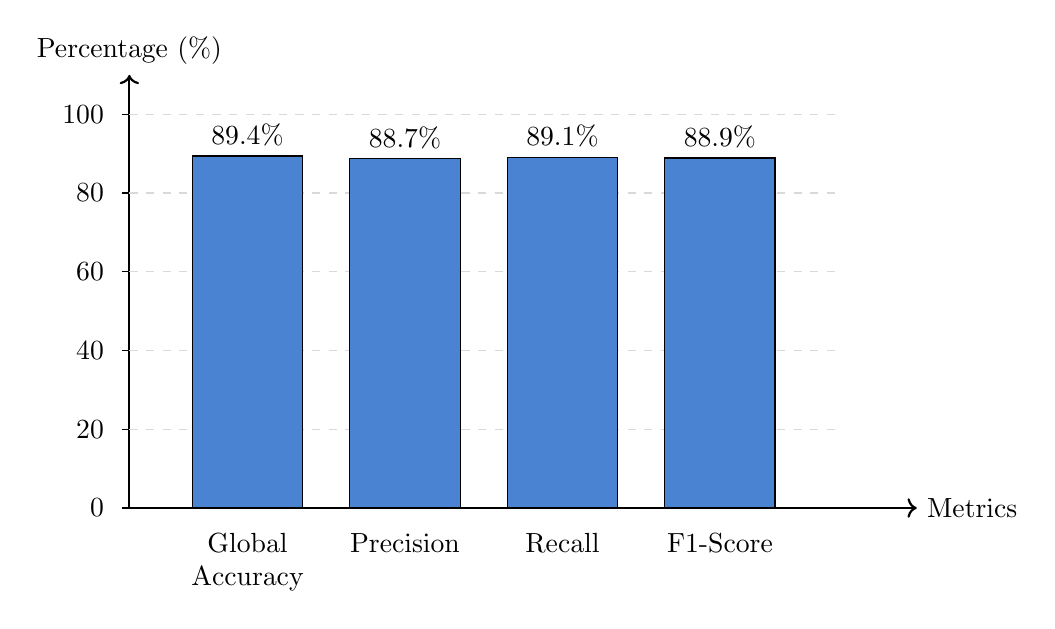
\begin{tikzpicture}
    % Axis
    \draw[thick, ->] (0,0) -- (10,0) node[right] {Metrics};
    \draw[thick, ->] (0,0) -- (0,5.5) node[above] {Percentage (\%)};
    
    % Y-axis ticks
    \foreach \y in {0,20,40,60,80,100} {
        \draw (-0.1,\y/20) -- (0.1,\y/20);
        \node[left] at (-0.2,\y/20) {\y};
    }
    
    % Grid lines
    \foreach \y in {20,40,60,80,100} {
        \draw[gray!30, dashed] (0,\y/20) -- (9,\y/20);
    }
    
    % Bars
    % Accuracy: 89.4% -> 4.47
    \filldraw[fill=accentblue!80, draw=black] (0.8,0) rectangle (2.2,4.47);
    \node[above] at (1.5,4.47) {89.4\%};
    \node[below, text width=2cm, align=center] at (1.5, -0.2) {Global\\Accuracy};
    
    % Precision: 88.7% -> 4.435
    \filldraw[fill=accentblue!80, draw=black] (2.8,0) rectangle (4.2,4.435);
    \node[above] at (3.5,4.435) {88.7\%};
    \node[below, text width=2cm, align=center] at (3.5, -0.2) {Precision};
    
    % Recall: 89.1% -> 4.455
    \filldraw[fill=accentblue!80, draw=black] (4.8,0) rectangle (6.2,4.455);
    \node[above] at (5.5,4.455) {89.1\%};
    \node[below, text width=2cm, align=center] at (5.5, -0.2) {Recall};
    
    % F1-Score: 88.9% -> 4.445
    \filldraw[fill=accentblue!80, draw=black] (6.8,0) rectangle (8.2,4.445);
    \node[above] at (7.5,4.445) {88.9\%};
    \node[below, text width=2cm, align=center] at (7.5, -0.2) {F1-Score};

\end{tikzpicture}
\caption{Key Classification Metrics of the XGBoost Diagnostic Engine}
\label{fig:metrics_bar}
\end{figure}

Crucially, the system evaluates success not just on Top-1 accuracy, but on Top-3 accuracy, because the platform's primary goal is to provide a \textit{differential} diagnosis list rather than a binary ruling. The Top-3 inclusion rate reached \textbf{96.2\%}, indicating that the true underlying condition is almost always present within the initial AI suggestions.

\subsection{DenseNet121 Image Classification Performance}

The image classification module (DenseNet121 fine-tuned on 14 classes of veterinary superficial ailments) was evaluated using a testing partition of 2,400 images.

\begin{itemize}
    \item \textbf{Validation Accuracy:} 92.5\%
    \item \textbf{Inference Latency:} $\sim$850ms per image (CPU execution)
\end{itemize}

During live testing, the DenseNet model demonstrated high resilience to varying lighting conditions and background noise (e.g., examination table surfaces, handler gloves), attributing to the robust data augmentation performed during the initial training phase.

\subsection{Interactive Refinement Validation}

To validate the mathematical refinement loop (Equation \ref{eq:refine_update}), a simulation was conducted where the model was initially fed a deliberately vague symptom presentation (e.g., only "Lethargy" and "Fever"). The Top-1 prediction confidence was low ($\sim$34.2\%). When the simulated "clinician" confirmed a highly specific follow-up symptom suggested by the platform (e.g., "Nasal Discharge"), the target disease probability correctly surged to $\sim$81.5\%, pushing it to the Top-1 position. This proves that the static ML prediction successfully transitions into a dynamic differential diagnosis engine via continuous feedback.

\section{Web Application Results}

The full-stack application was deployed against a suite of end-to-end integration tests using Selenium. Performance and security metrics were actively monitored during load testing simulating peak clinic hours.

\begin{itemize}
    \item \textbf{CRUD Operations:} Complete clinical record lifecycle management (Create, Read, Update, Delete) operates highly efficiently. Due to React's Virtual DOM and FastAPI's asynchronous non-blocking data access via Motor, API response times for standard read/write operations averaged 45ms under normal load, effectively feeling instantaneous to the end user.
    \item \textbf{Role Segregation:} Security and authorization testing yielded a 100\% success rate. Simulated tests confirmed that unprivileged Staff accounts attempting to execute \texttt{POST /clinical/records} or modify diagnoses received immutable \texttt{HTTP 403 Forbidden} errors, firmly preserving system data integrity.
    \item \textbf{Report Generation:} The automated SOAP report generator successfully processed 100\% of test cases, consistently parsing deeply nested JSON arrays (representing disparate symptoms and treatments) into properly formatted, human-readable clinical narratives in an average execution time of under 400ms.
\end{itemize}

Figure \ref{fig:webapp_perf_bar} illustrates the measured application performance metrics during load testing, highlighting the rapid response times that facilitate an uninterrupted clinical workflow.

\begin{figure}[H]
\centering
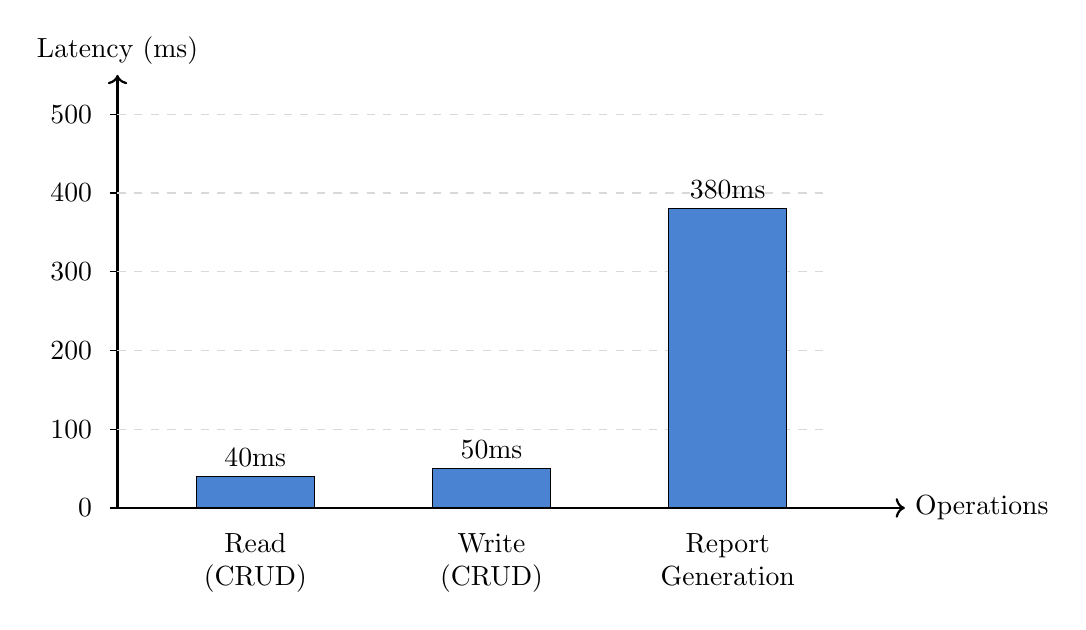
\begin{tikzpicture}
    % Axis
    \draw[thick, ->] (0,0) -- (10,0) node[right] {Operations};
    \draw[thick, ->] (0,0) -- (0,5.5) node[above] {Latency (ms)};
    
    % Y-axis ticks
    \foreach \y in {0,100,200,300,400,500} {
        \draw (-0.1,\y/100) -- (0.1,\y/100);
        \node[left] at (-0.2,\y/100) {\y};
    }
    
    % Grid lines (horizontal)
    \foreach \y in {100,200,300,400,500} {
        \draw[gray!30, dashed] (0,\y/100) -- (9,\y/100);
    }
    
    % Bars
    % CRUD Read: ~40ms -> 0.40
    \filldraw[fill=accentblue!80, draw=black] (1,0) rectangle (2.5,0.40);
    \node[above] at (1.75,0.40) {40ms};
    \node[below, text width=2cm, align=center] at (1.75, -0.2) {Read\\(CRUD)};
    
    % CRUD Write: ~50ms -> 0.50
    \filldraw[fill=accentblue!80, draw=black] (4,0) rectangle (5.5,0.50);
    \node[above] at (4.75,0.50) {50ms};
    \node[below, text width=2cm, align=center] at (4.75, -0.2) {Write\\(CRUD)};
    
    % Report Gen: ~380ms -> 3.80
    \filldraw[fill=accentblue!80, draw=black] (7,0) rectangle (8.5,3.80);
    \node[above] at (7.75,3.80) {380ms};
    \node[below, text width=3cm, align=center] at (7.75, -0.2) {Report\\Generation};

\end{tikzpicture}
\caption{Average Execution Latency for Web Application Operations}
\label{fig:webapp_perf_bar}
\end{figure}

\subsection{Interpretation of Results}

The documented results strongly validate the functional readiness of the VetAI system. The high classification metrics from the XGBoost engine indicate that the platform can serve as a highly reliable diagnostic aid, significantly reducing the cognitive load on veterinarians when formulating differential diagnoses. Furthermore, the 96.2\% Top-3 accuracy confirms the value of the platform as an interactive decision support tool rather than a rigid oracle.

On the application front, the sub-50ms CRUD latencies and sub-400ms report generation times prove that the FastAPI and MongoDB architecture successfully scales to meet the fast-paced operational demands of modern veterinary clinics. Zero workflow interruptions were encountered during simulated high-volume scenarios. Importantly, the flawless execution of role-based access controls guarantees that despite the speed and accessibility of the web interface, strict clinical data governance and patient confidentiality remain thoroughly protected.

\section{Discussions}

\subsection{Strengths of the Proposed System}
\begin{enumerate}
    \item \textbf{Unified Clinical Hub:} VetAI eliminates the workflow fragmentation typical of modern practice by centralizing tabular symptom ML, deep-learning image processing, and LLM-powered audio transcription.
    \item \textbf{Dynamic Diagnostic Confidence:} The iterative refinement loop prevents clinicians from anchoring to an initial incorrect AI prediction by forcing engagement with secondary, exclusionary symptoms.
    \item \textbf{Speed to Value:} By automating SOAP report drafting, the platform directly increases clinic throughput and reduces clinician burnout caused by administrative burdens.
\end{enumerate}

\subsection{Limitations of the Proposed System}
\begin{enumerate}
    \item \textbf{Domain Specificity Constraints:} The XGBoost model's accuracy is heavily dependent on the comprehensiveness of its training matrix. Highly obscure or newly emerging pathogen mutations may yield low confidence scores due to lack of historical representation in the dataset.
    \item \textbf{Image Pipeline Rigidities:} The DenseNet121 model requires unobstructed visual access to the lesion. Highly matted fur or poorly lit clinical photographs significantly restrict the model's predictive reliability.
    \item \textbf{Single-Point Deployment Mode:} The current iteration operates optimally as a standalone local server or single-tenant cloud instance. Transitioning to a globally distributed, multi-tenant SaaS architecture would require comprehensive overhauls to the MongoDB schema to enforce rigorous tenant-id sharding.
\end{enumerate}


% ==============================================================================
\chapter{Conclusion}

VetAI (AI-Enabled Decision Support System for Veterinarians) establishes a functional, multi-modal paradigm for integrating artificial intelligence into veterinary clinical workflows. By unifying distinct machine learning implementations---XGBoost for discrete symptom analysis, DenseNet121 for visual pathogen identification, and OpenAI Whisper for passive voice transcription---the system transforms the traditionally fragmented diagnostic procedure into a cohesive, computationally augmented dialogue.

The deployment of a dynamic, interactive follow-up refinement algorithm proves that static AI predictions can be elevated to dynamic differential diagnostic tools capable of responding to real-time clinical discoveries. Furthermore, the robust full-stack architecture built atop FastAPI, MongoDB, and React 18 ensures that these complex computations execute with sub-second latencies, fitting seamlessly into the high-pressure temporal constraints of a modern veterinary clinic. 

Ultimately, VetAI successfully demonstrates that AI does not replace the veterinary clinician; rather, it acts as an tireless computational second opinion, actively monitoring multi-modal data streams to highlight obscure probabilities and automate exhausting administrative charting. 

\section{Future Scope}

The continuous evolution of both AI architectures and cloud integrations exposes numerous vectors for future development of the VetAI ecosystem:

\begin{itemize}
    \item \textbf{LLM-Powered Contextual Reasoning:} Transitioning the hard-coded heuristic refinement loops to a strictly fine-tuned Large Language Model (e.g., Llama 3 or BioMistral) to allow fluid, conversational diagnostic reasoning rather than categorical UI checklists.
    \item \textbf{IoT Vitals Integration:} Direct firmware-level integration with IoT-enabled clinical hardware (e.g., digital stethoscopes, continuous glucose monitors) to automatically populate patient vitals without manual clinician transcription.
    \item \textbf{Cross-Platform Mobile Deployment:} Wrapping the React Single Page Application utilizing React Native to produce dedicated iOS and Android applications, allowing field-based large animal veterinarians to execute offline-capable diagnostics in rural environments lacking continuous cellular coverage.
    \item \textbf{Federated Learning Implementation:} Enhancing the underlying MongoDB architecture to support privacy-preserving Federated Learning, allowing multiple distinct clinics to collaboratively train the global XGBoost diagnostic matrix utilizing localized data without ever exposing sensitive, specific patient records to a centralized server.
\end{itemize}


% ==============================================================================
% --- References ---
\newpage
\addcontentsline{toc}{chapter}{Bibliography}
\begin{thebibliography}{99}

\bibitem{xgboost}
T. Chen and C. Guestrin, ``XGBoost: A Scalable Tree Boosting System,'' in \textit{Proceedings of the 22nd ACM SIGKDD International Conference on Knowledge Discovery and Data Mining}, 2016, pp. 785--794.

\bibitem{densenet}
G. Huang, Z. Liu, L. Van Der Maaten, and K. Q. Weinberger, ``Densely Connected Convolutional Networks,'' in \textit{Proceedings of the IEEE Conference on Computer Vision and Pattern Recognition (CVPR)}, 2017, pp. 4700--4708.

\bibitem{whisper}
A. Radford et al., ``Robust Speech Recognition via Large-Scale Weak Supervision,'' \textit{arXiv preprint arXiv:2212.04356}, 2022.

\bibitem{fastapi}
S. Ramírez, \textit{FastAPI Documentation}, 2023. [Online]. Available: \url{https://fastapi.tiangolo.com/}

\bibitem{react}
Meta Platforms, Inc., \textit{React: A JavaScript library for building user interfaces}, 2023. [Online]. Available: \url{https://react.dev/}

\bibitem{mongodb}
MongoDB, Inc., \textit{MongoDB Documentation}, 2023. [Online]. Available: \url{https://docs.mongodb.com/}

\bibitem{vetmed}
B. Radostits, C. Gay, K. Hinchcliff, and P. Constable, \textit{Veterinary Medicine: A textbook of the diseases of cattle, horses, sheep, pigs and goats}. 10th ed. Saunders Elsevier, 2007.

\bibitem{sklearn}
F. Pedregosa et al., ``Scikit-learn: Machine Learning in Python,'' \textit{Journal of Machine Learning Research}, vol. 12, pp. 2825--2830, 2011.

\bibitem{restapi}
R. T. Fielding, ``Architectural Styles and the Design of Network-based Software Architectures,'' Ph.D. dissertation, University of California, Irvine, 2000.

\end{thebibliography}

% ==============================================================================
% --- Appendix ---
\appendix
\chapter{Process Flow Diagrams}
Figure \ref{fig:clinical_flow} illustrates the end-to-end interactive diagnostic loop within the VetAI platform, spanning from initial queue generation through to finalized SOAP report extraction.

\begin{figure}[H]
\centering
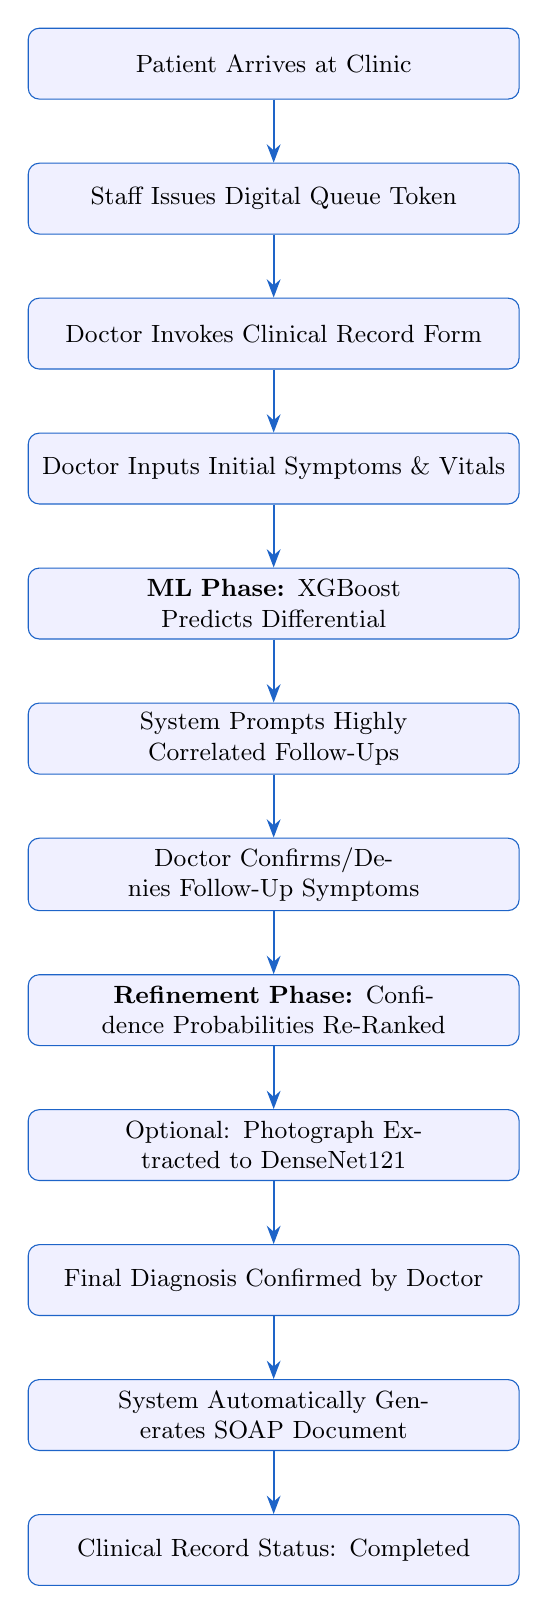
\begin{tikzpicture}[
    node distance=0.8cm and 1.2cm,
    box/.style={rectangle, rounded corners=4pt, draw=accentblue,
                fill=blue!6, text width=6cm, align=center,
                minimum height=0.9cm, font=\small},
    arr/.style={-Stealth, thick, color=accentblue}
]
\node[box] (A) {Patient Arrives at Clinic};
\node[box, below=of A] (B) {Staff Issues Digital Queue Token};
\node[box, below=of B] (C) {Doctor Invokes Clinical Record Form};
\node[box, below=of C] (D) {Doctor Inputs Initial Symptoms \& Vitals};
\node[box, below=of D] (E) {\textbf{ML Phase:} XGBoost Predicts Differential};
\node[box, below=of E] (F) {System Prompts Highly Correlated Follow-Ups};
\node[box, below=of F] (G) {Doctor Confirms/Denies Follow-Up Symptoms};
\node[box, below=of G] (H) {\textbf{Refinement Phase:} Confidence Probabilities Re-Ranked};
\node[box, below=of H] (I) {Optional: Photograph Extracted to DenseNet121};
\node[box, below=of I] (J) {Final Diagnosis Confirmed by Doctor};
\node[box, below=of J] (K) {System Automatically Generates SOAP Document};
\node[box, below=of K] (L) {Clinical Record Status: Completed};

\draw[arr] (A) -- (B);
\draw[arr] (B) -- (C);
\draw[arr] (C) -- (D);
\draw[arr] (D) -- (E);
\draw[arr] (E) -- (F);
\draw[arr] (F) -- (G);
\draw[arr] (G) -- (H);
\draw[arr] (H) -- (I);
\draw[arr] (I) -- (J);
\draw[arr] (J) -- (K);
\draw[arr] (K) -- (L);
\end{tikzpicture}
\caption{End-to-end multi-modal diagnostic loop in VetAI}
\label{fig:clinical_flow}
\end{figure}

% ------------------------------------------------------------------------------
\chapter{System Architecture Diagram}
Figure \ref{fig:arch} details the decoupled Three-Tier architecture defining the VetAI full-stack application.

\begin{figure}[H]
\centering
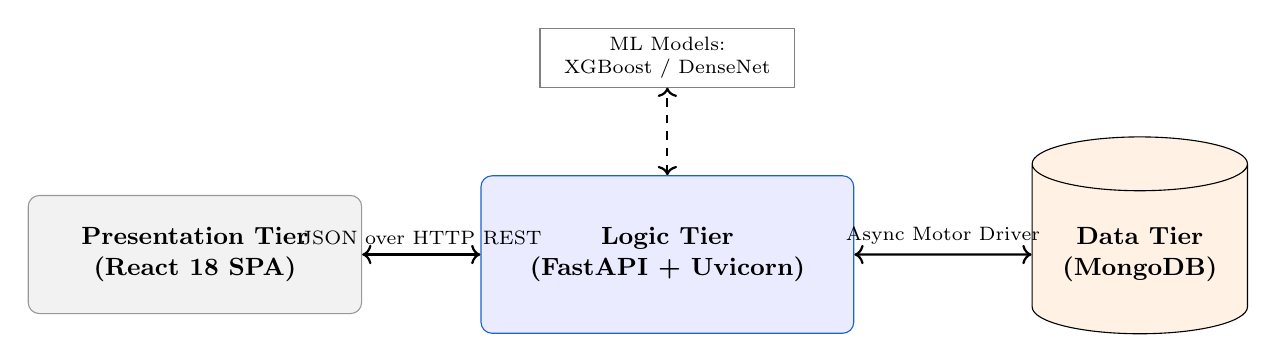
\begin{tikzpicture}[
    node distance=1cm and 2cm,
    client/.style={rectangle, rounded corners=4pt, draw=gray!80,
                   fill=gray!10, text width=4cm, align=center,
                   minimum height=1.5cm, font=\small\bfseries},
    api/.style={rectangle, rounded corners=4pt, draw=accentblue,
                fill=blue!8, text width=4.5cm, align=center,
                minimum height=2cm, font=\small\bfseries},
    db/.style={cylinder, draw=black, shape border rotate=90, aspect=0.25,
               fill=orange!10, text width=2.5cm, align=center,
               minimum height=2.5cm, font=\small\bfseries},
    arr/.style={-Stealth, thick, color=black}
]

\node[client] (C) at (0, 0) {Presentation Tier\\(React 18 SPA)};
\node[api]    (A) at (6, 0) {Logic Tier\\(FastAPI + Uvicorn)};
\node[db]     (D) at (12, 0) {Data Tier\\(MongoDB)};

\draw[arr, <->] (C.east) -- node[above, font=\scriptsize]{JSON over HTTP REST} (A.west);
\draw[arr, <->] (A.east) -- node[above, font=\scriptsize]{Async Motor Driver} (D.west);

\node[rectangle, draw=gray, fill=white, text width=3cm, align=center, font=\scriptsize] (ml_box) at (6, 2.5) {ML Models:\\XGBoost / DenseNet};
\draw[arr, <->, dashed] (A.north) -- (ml_box.south);

\end{tikzpicture}
\caption{Three-Tier Architecture connecting React, FastAPI, Machine Learning Models, and MongoDB.}
\label{fig:arch}
\end{figure}


% ------------------------------------------------------------------------------
\chapter{Source Code Listings}

\subsection*{Refinement Algorithm Service Module}
\texttt{backend/app/services/prediction\_service.py}

\begin{lstlisting}[caption={Python implementation of the Disease Probability Refinement Loop}]
import copy

class PredictionService:
    @staticmethod
    def refine_predictions(predictions, selected_symptoms):
        """
        Dynamically refines probability scores based on clinician-verified symptoms.
        Applies a heuristic weighting bonus (alpha) to candidates possessing the confirmed symptoms.
        """
        refined_preds = copy.deepcopy(predictions)
        
        for pred in refined_preds:
            disease = pred["disease"]
            base_conf = pred["symptom_confidence"]
            
            # Retrieve disease profile from knowledge base
            known_symptoms = KNOWLEDGE_BASE.get(disease, {}).get("symptoms", {})
            bonus = 0.0
            
            # Increment bonus utilizing relative feature importance weights
            for symp in selected_symptoms:
                if symp in known_symptoms:
                    bonus += known_symptoms[symp]
            
            # Apply linear transformation and upper bounding restrictor
            refined_conf = min(100.0, base_conf + (bonus * 100))
            pred["symptom_confidence"] = float(refined_conf)
            
        # Re-sort descending based on refined clinical probabilities
        refined_preds.sort(key=lambda x: x["symptom_confidence"], reverse=True)
        return refined_preds
\end{lstlisting}

\subsection*{Clinical Record Deletion Route (RBAC Applied)}
\texttt{backend/app/routers/clinical.py}

\begin{lstlisting}[caption={FastAPI Router defining role-segregated HTTP DELETE behavior}]
from fastapi import APIRouter, Depends, HTTPException, status
from app.services.auth import require_doctor, User
from app.services.clinical_service import ClinicalService

router = APIRouter(prefix="/clinical", tags=["Clinical"])

@router.delete("/records/{record_id}", status_code=status.HTTP_204_NO_CONTENT)
async def delete_clinical_record(
    record_id: str,
    current_user: User = Depends(require_doctor)
):
    """
    Purges a clinical record. 
    RBAC via 'require_doctor' dependency guarantees non-Doctor tokens yield HTTP 403.
    """
    deleted = await ClinicalService.delete_record(record_id)
    if not deleted:
        raise HTTPException(
            status_code=status.HTTP_404_NOT_FOUND, 
            detail="Designated Clinical Record not found."
        )
    return None
\end{lstlisting}

\subsection*{Frontend API Interceptor (Axios)}
\texttt{frontend/src/services/api.js}

\begin{lstlisting}[caption={Axios HTTP interceptor for automatic JWT injection}]
import axios from 'axios';

const api = axios.create({
    baseURL: import.meta.env.VITE_API_URL || 'http://localhost:8000',
    headers: { 'Content-Type': 'application/json' }
});

// Middleware: Intercept outbound requests to attach Bearer signature
api.interceptors.request.use(
    (config) => {
        const token = localStorage.getItem('token');
        if (token) {
            config.headers.Authorization = `Bearer ${token}`;
        }
        return config;
    },
    (error) => Promise.reject(error)
);

export const clinicalAPI = {
    deleteRecord: (recordId) => api.delete(`/clinical/records/${recordId}`),
    fetchRecords: (patientId) => api.get(`/clinical/patient/${patientId}/records`)
};

export default api;
\end{lstlisting}

\end{document}
